\documentclass[a4paper,12pt]{article}

%%% Работа с русским языком
\usepackage{cmap}					% поиск в PDF
\usepackage{mathtext} 				% русские буквы в формулах
\usepackage[T2A]{fontenc}			% кодировка
\usepackage[utf8]{inputenc}			% кодировка исходного текста
\usepackage[english,russian]{babel}	% локализация и переносы
\usepackage{xcolor}
\usepackage{hyperref}
 % Цвета для гиперссылок
\definecolor{linkcolor}{HTML}{00FFFF} % цвет ссылок
\definecolor{urlcolor}{HTML}{4682B4} % цвет гиперссылок

\hypersetup{pdfstartview=FitH,  linkcolor=linkcolor,urlcolor=urlcolor, colorlinks=true}

%%% Дополнительная работа с математикой
\usepackage{amsfonts,amssymb,amsthm,mathtools} % AMS
\usepackage{amsmath}
\usepackage{icomma} % "Умная" запятая: $0,2$ --- число, $0, 2$ --- перечисление

%% Номера формул
%\mathtoolsset{showonlyrefs=true} % Показывать номера только у тех формул, на которые есть \eqref{} в тексте.

%% Шрифты
\usepackage{euscript}	 % Шрифт Евклид
\usepackage{mathrsfs} % Красивый матшрифт

%% Свои команды
\DeclareMathOperator{\sgn}{\mathop{sgn}}

\usepackage{enumerate}
%% Перенос знаков в формулах (по Львовскому)
\newcommand*{\hm}[1]{#1\nobreak\discretionary{}
{\hbox{$\mathsurround=0pt #1$}}{}}
% графика
\usepackage{graphicx}
\graphicspath{{picture/}}
\DeclareGraphicsExtensions{.pdf,.png,.jpg}
\author{Бурмашев Григорий, 208. \href{https://teleg.run/burmashev}{@burmashev}}
\title{Дискретная математика. Коллок -- 1. Определения и задачи по ним.}
\date{}
\begin{document}
\section*{Задание 1}
Все возможные случаи описаны на картинке. Ну а решений больше 6 у нас быть не может, т.к $C_4^2 = \frac{12}{2} = 6$
\begin{center}
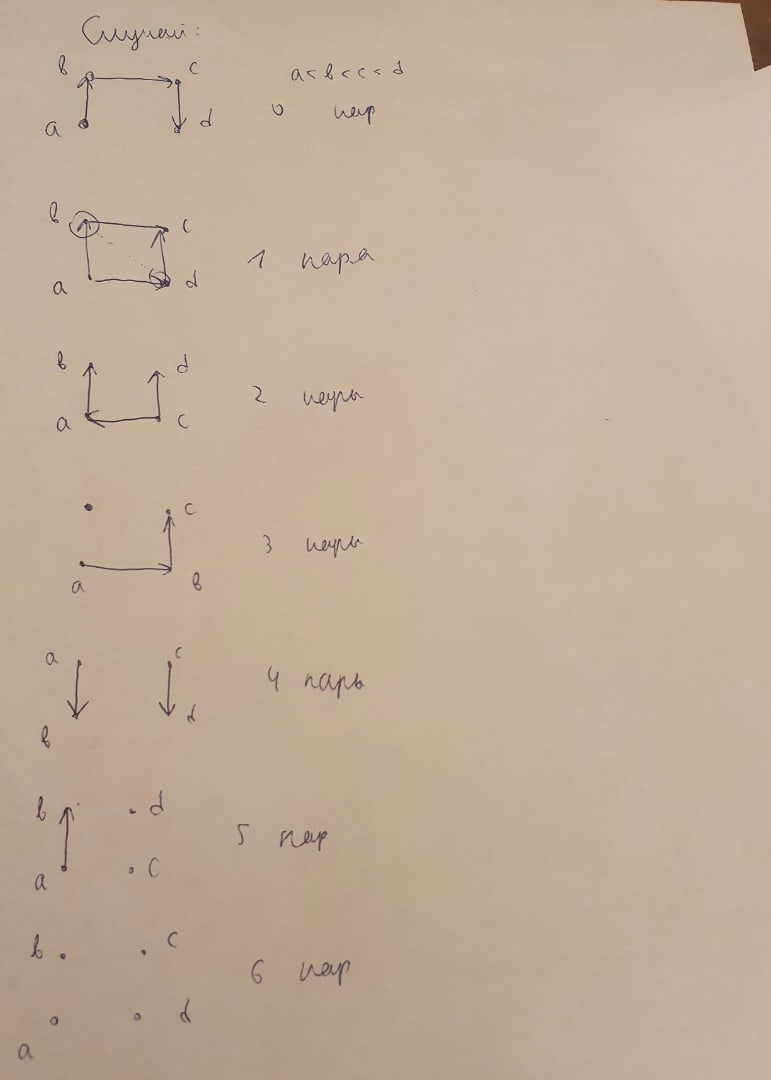
\includegraphics[scale=0.4]{1Gxl2kd-6LU.jpg}
\end{center}
\newpage
\section*{Задание 2}
Решение на рисунке:
\begin{center}
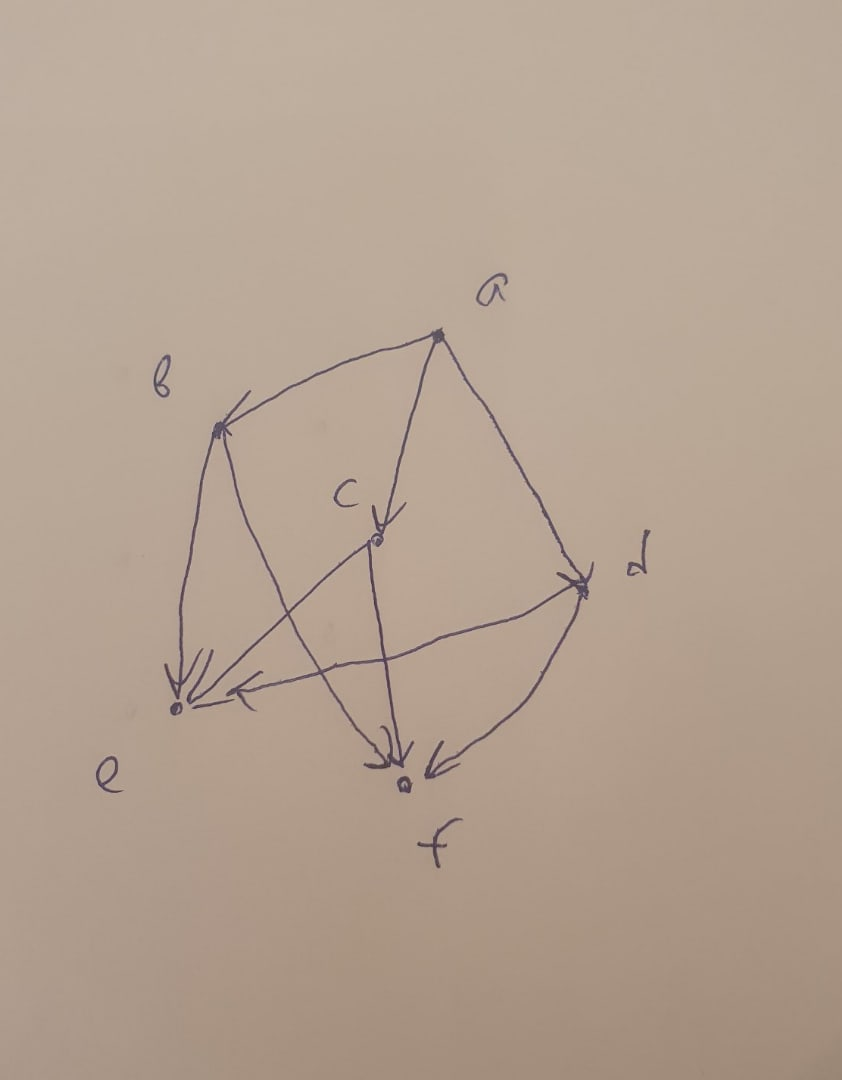
\includegraphics[scale=0.4]{65AQJAscBXI.jpg}
\end{center}
\newpage
\section*{Задание 3}
Решение на рисунке (ребра в соотвествии с условияеми $x \subseteq y$ и с делимостью):
\begin{center}
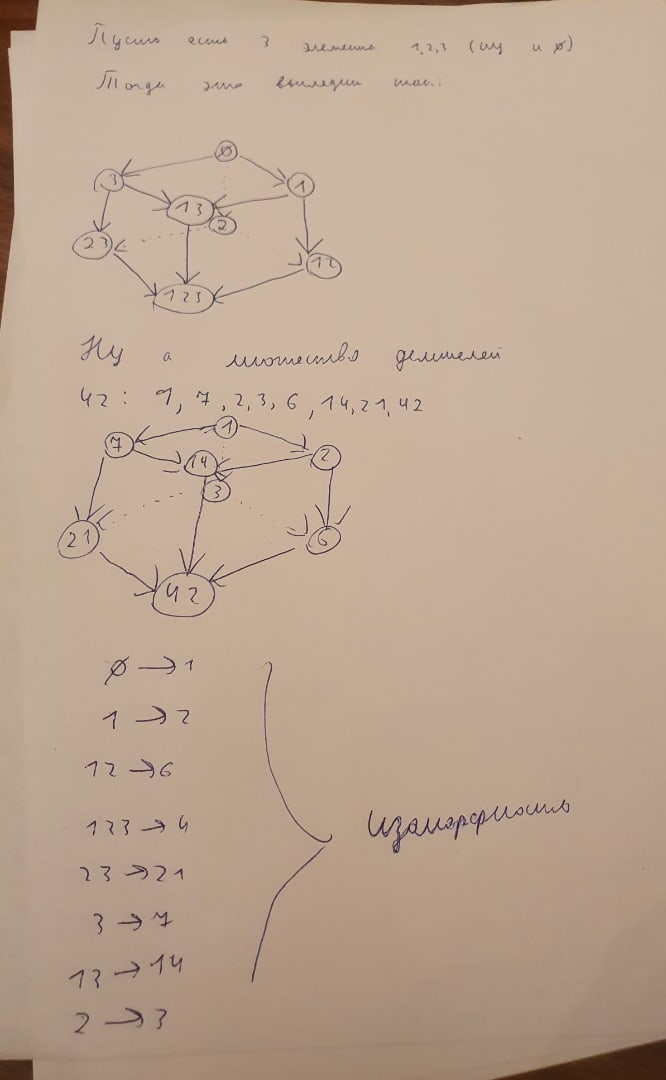
\includegraphics[scale=0.4]{7yVZbj5okUA.jpg}
\end{center}
\end{document}
